
%\renewcommand{\familydefault}{\sfdefault}
%=============== En−Tete ===============
 
%−−− Insertion de paquetages −−−−
\documentclass[12pt,a4paper,french]{report}
\usepackage[utf8]{inputenc}
\usepackage{amsmath}
\usepackage{amsfonts}
\usepackage{amssymb}
\usepackage{graphicx}
\usepackage{wrapfig}
\graphicspath{ {./images/} }
\usepackage[rightcaption]{sidecap}
\usepackage{subcaption}


\usepackage[french]{babel}
\usepackage[Bjarne]{fncychap}
\usepackage{fancyhdr}
\usepackage{float}
\usepackage{epsfig}
\usepackage{appendix}
\usepackage[final]{pdfpages}
\usepackage{array}
\usepackage{pdfpages}
\usepackage{hyperref}

\pagestyle{fancy}
\usepackage{titlesec}


%-\titleformat{\chapter}[display]{\bfseries}{\huge\chaptertitlename~\thechapter}{10pt}{\LARGE}--%

%−−− Page de garde - titre −−−

\begin{document}

\title{\Large{\Large {Travail de lecture et de rédaction scientifique sur le Federate Learning}}}

\author{Bal Sébastien}

\maketitle

\thispagestyle{empty} % Ignore page number

 

%=============== Remerciement ===============

\begin{figure}[p]

\large\textbf{Remerciements}


Je tiens à remercier toutes les personnes qui m'ont aidé lors de la rédaction de ce rapport. Ainsi que les personnes qui m'ont conseillé et relu lors de la rédaction de ce rapport : ma famille et mon meilleur ami Benjamin B. 

\end{figure}

\tableofcontents
\thispagestyle{empty} % Ignore page number




\chapter{Introduction}

\fancyfoot[C]{Master en Science infomatique - Lecture et rédaction scientifique}

\fancyhead[R]{\textbf{Chaptire \thechapter}}
\fancyfoot[R]{\thepage}

Notre monde comme nous le connaissons devient de plus en plus connecté, chaque seconde 29 000 Gigaoctets d'informations sont publiées dans le monde. Cette quantité doit être exploitée, bien entendu pas comme l'a fait Facebook, avec le scandale Facebook-Cambridge le jour des élections aux Etats Unis. Il y a de meilleures solutions pour utiliser ces données, prenons la recherche médicale améliorer la localisation de maladie. Ou bien dans la finance avec des calculs pour prédire les futurs entreprises florissantes. Tant de possibilités a exploiter, mais des méthodes sont apparues pour exploiter ces données. On débutera avec l'explication du concept de Machine Learning. Puis plus en profondeur, le Deep Learning. Et pour finir, le Federated Learning avec ses données et ses modèles décentralisées.





%\thispagestyle{plain}
\setcounter{page}{1} % Start page count

\chapter{Machine Learning}
Le Machine Learning appelé en Français apprentissage automatique "[...] est un champ d'étude de l'intelligence artificielle qui se fonde sur des approches mathématiques et statistiques pour donner aux ordinateurs la capacité d'apprendre à partir de données[...]".Ceci a pour objectif de traiter l'information afin de lui donner de la valeur ajoutée.\\

De nos jours, le Machine Learning est présent partout sur la toile, cela va du moteur de recherche comme Google, aux assistants vocaux comme Siri et Alexa, les fils d'actualités des réseaux sociaux comme Facebook et Twitter. Le point commun entre toutes ces platformes et le stockage massif des données de leur utilisateur appelé Big Data, comme le site du dictionnaire Larousse, "c'est un domaine technologique dédié à l'analyse de très grands volumes de données informatiques". Le Big Data est une technologie apparue dans les années 1900, elle a permis l'essor de l'apprentissage automatique, le Machine Learning. En effet, cet imposant volume de données collectées sur les utilisateurs a permis, dans les exemples cités ci-dessus, de mieux cibler le comportement des utilisateurs et ainsi améliorer les expériences.\\

Pour fonctionner, le Machine Learning(ML) a besoin de données à ingérer et d'un modèle appris afin de fournir des données à valeur ajoutée comme des algorithmes de prédiction de bourse et la maintenance prédictive. Il est donc nécessaire d'identifier les approches techniques pour créer ces modèles de ML.\\

\begin{center}
	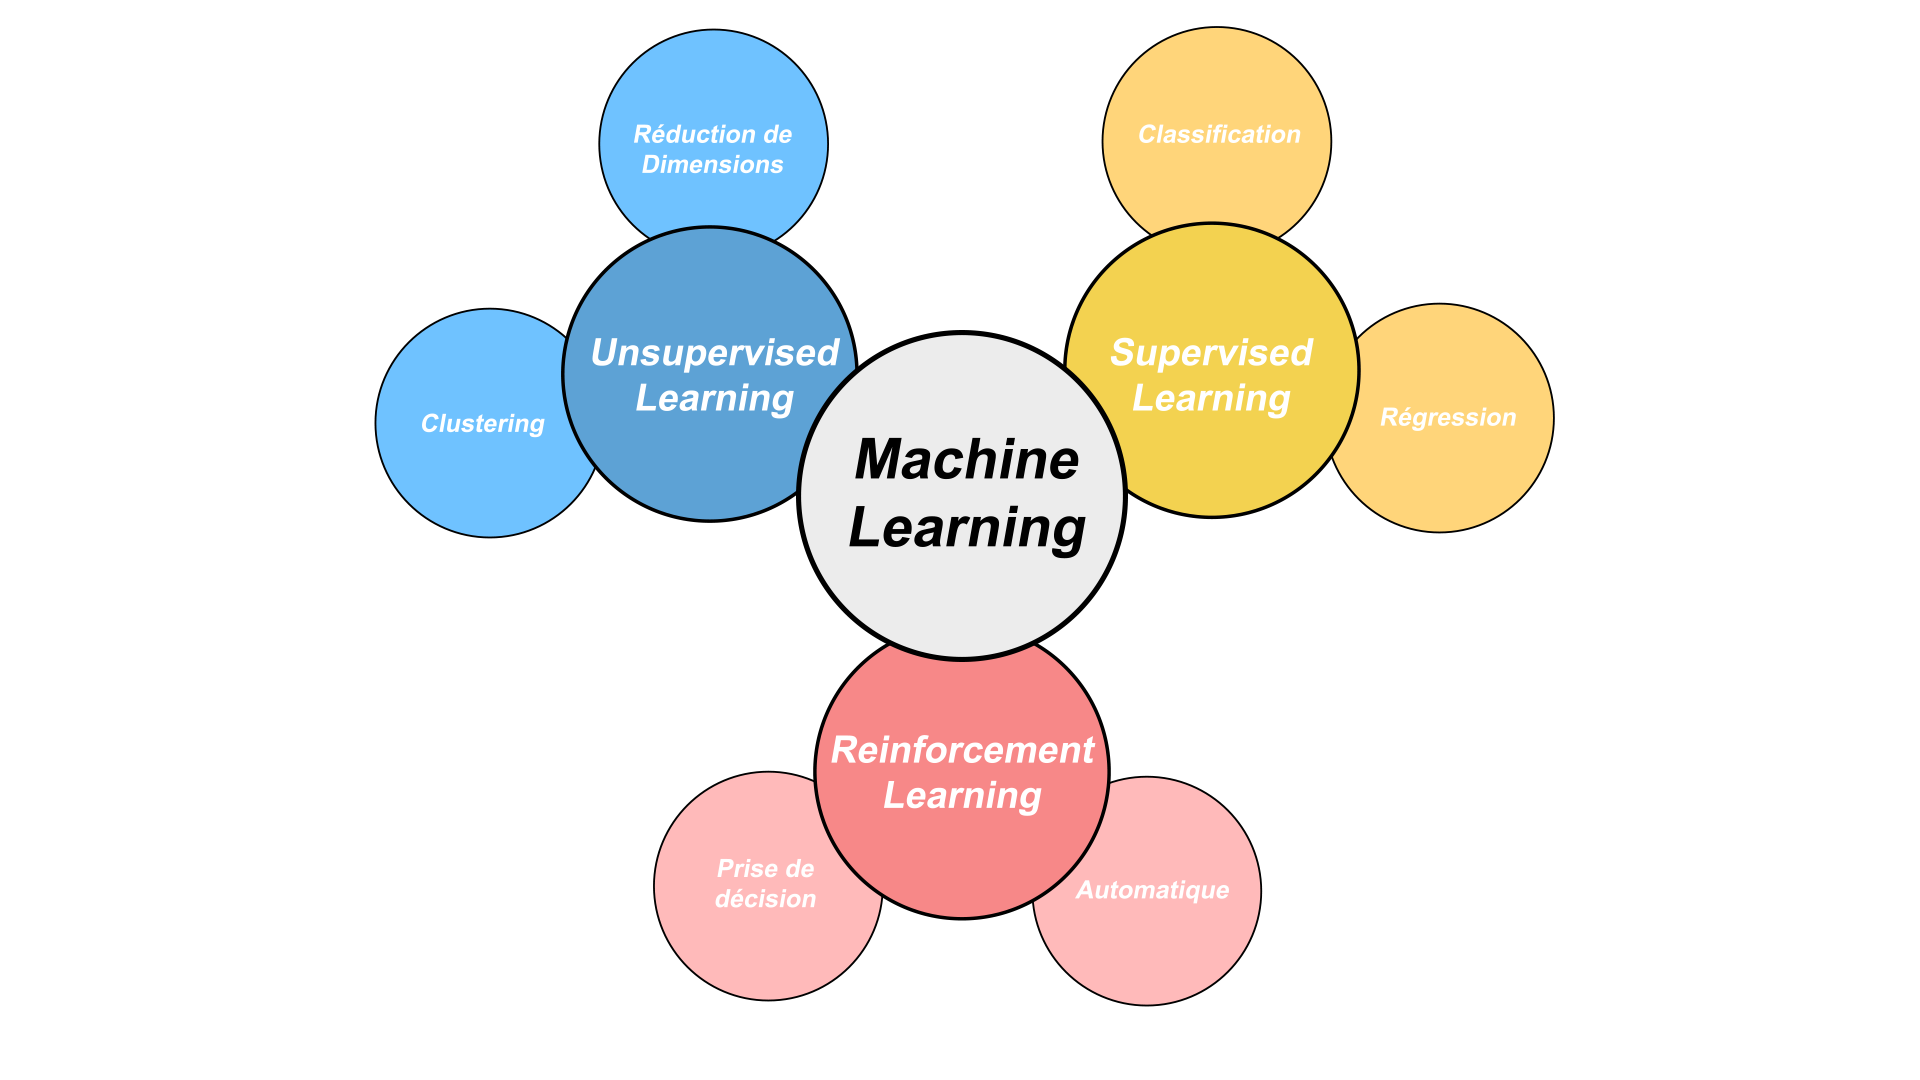
\includegraphics[scale=0.2]{ML_vignette}
	\captionof{figure}{Familles d'algorithmes les plus utilisés}
	\label{fig1}
\end{center}

La première famille, l'apprentissage supervisé (en jaune dans la figure 1.1) consiste à fournir des données en entrées, le résultat attendu itéré sur un grand jeu de données afin de trouver le modèle. Pour que le modèle devienne performant, on fournit un grand volume de données dans le but qu'il se rapproche du modèle attendu. Ce type de modèle nécessite donc une bonne connaissance du processus métier vu qu'il est nécessaire de fournir des jeux de données en entrées pour obtenir le résultat désiré. Ce type de modèle est donc souvent utilisé pour simplifier ou optimiser des solutions existantes.\\

En prenant l'algorithme de l'arbre de classification et de régression, on peut constater que les données suivent un chemin qui a été défini au préalable par un développeur. Dans la fig 1.2, on peut remarquer le cheminement de l'algorithme sur un jeu de données.

\begin{center}
	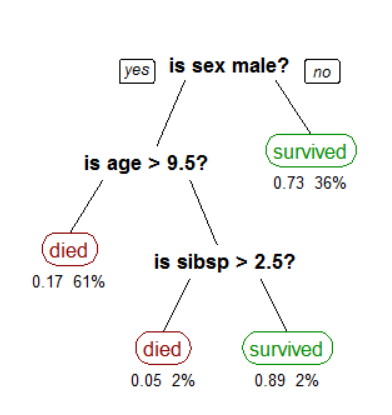
\includegraphics[scale=0.5]{ML_superviser}
	\captionof{figure}{Abre de classiffication et de régression}
	\label{fig1}
\end{center}


La deuxième famille, l'apprentissage non-surpervisé (en bleu dans la figure 1.1) consiste à apprendre par identification des ressemblances et des différences entre les données fournies. L'algorithme rassemble les données en groupes ce qui permet, lors de l'intégration d'une nouvelle information, de la classifier dans un des groupes existants très rapidement. Ce type d'exemple a souvent pour objectif de créer des arbres de décisions sur base de "clustering".
Un des plus connus est le partitionnement k-means, c'est un algorithme qui met en place un centre de gravité, dont les coordonnées vont servir pour localiser cette zone. Pour mieux comprendre l'algorithme, la notation $c^{(i)}$ représente la partition de point i et $u_j$ représente le centre de la partition j. L'algorithme k-means répète l'étape suivante jusqu'à sa convergence fig 1.3.\\

\begin{center}
	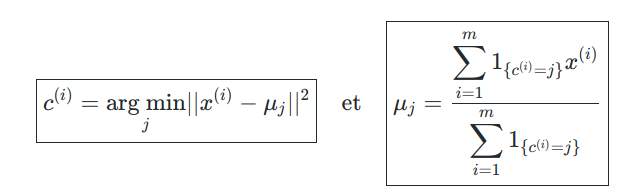
\includegraphics[scale=0.5]{algo_k_means}
	\captionof{figure}{Algorithme k-means}
	\label{fig1}
\end{center}
\pagebreak
Dans la fig 1.4, l'algorithme trie les données pour arriver à une convergence des données.

\begin{center}
	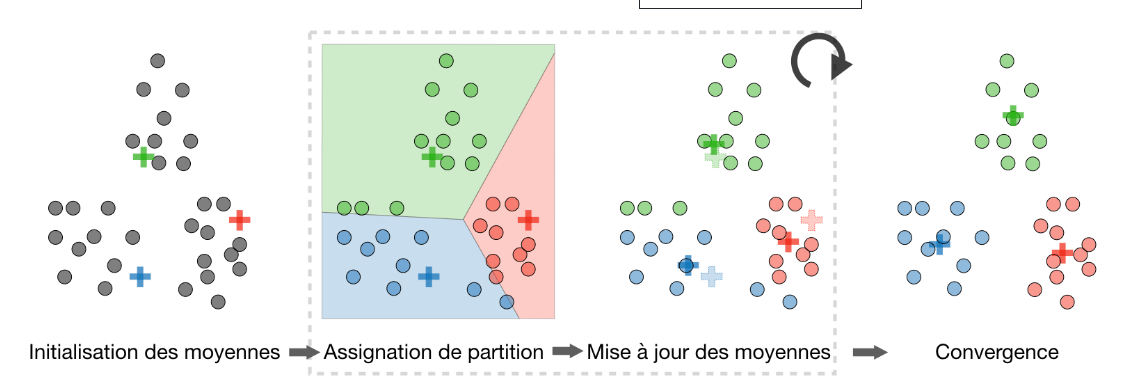
\includegraphics[scale=0.4]{k_means}
	\captionof{figure}{Shema k-means}
	\label{fig1}
\end{center}

Pour finir, il existe une catégorie qui gère sa propre expérience. En effet, l'apprentissage par renforcement (en rouge dans la figure 1.1) consiste à générer ses propres expériences. On se rapproche de l'automobile autonome, la machine change ses états suivant les actions qu'elle entreprend de faire. Un système de récompense positive ou négative est mis en place pour constituer une nouvelle expérience et inciter la machine attentive à maximiser ses chances de réussite. Ce type d'approche est la plus générique, elle convient aussi bien pour optimiser des solutions existantes que pour classifier des données. En règle générale, cette approche est souvent utilisée pour des recherches exploratoires. L'inconvénient principal de cettre approche scientifique est son besoin de ressources. En effet, les combinatoires peuvent très vite être importantes et pas conséquent, l'exploration aura besoin de temps ou de ressources physiques pour les tester.\\

Pour conclure, le ML est une technologie qui vise à trouver des modèles, comprendre des comportements afin de prédire les besoins d'une application suivant un la tâche à réaliser.\\

On peut constater que ce type de besoin se focalise sur une application spécifique cependant, le ML connaît des limites au niveau des complexités combinatoires [x: ]. Or certaines applications nécessitent des applications plus complexes avec plus d'entrées, telles que le traitement des images. Pour pallier les limites du ML, le Deep Learning a été développé.


\chapter{Deep Learning}

Le Deep Learning(DL) est représentatif d'un système neuronal comme notre système cérébral, il est conçu de plusieurs neurones qui interagissent entre eux. Pour rendre performants tous ces neurones, il est nécessaire d'avoir une grande quantité de données, un Data Lake. Celui-ci fournit au système plusieurs informations afin de lui constituer une "mémoire". Cette mémoire lui permet de reconnaître des éléments bien particuliers suivant l'entrainement qu'il aura suivi. Cet entrainement est supervisé par des développeurs qui vérifient que le DL ne sort pas de son modèle défini.
Si il s'en éloigne, ils corrigent son algorithme mathématique pour le rendre plus performant et le remettre sur le droit chemin. Pour que le modèle mathématique devienne performant, il faudra l'entrainer à reconnaître une donnée en particulier. C'est le sujet de notre prochaine section.


\section{Modèle d'entrainement}

Pour entrainer le DL, il lui faut un algorithme mathématique et un grand flux de données qu'il affine ses recherches et acquière de l'expérience. Dans notre situation, on décide de travailler sur la reconnaissance d'une image, en particulier celle d'un chat.
On fournit à l'algorithme un flux d'images de plusieurs espèces d'animaux, on définit les paramètres qui permettent d'affirmer que l'image que l'on soumet est bien un chat. Ainsi avec ces critères, l'algorithme devient plus précis car on le guide un peu sur l'objectif qu'il doit atteindre.
 
Voici un schéma pour l'exemple du fonctionnement du DL,[fig3.1] : les boules vertes représentent le bon chemin que le système va prendre pour arriver à vérifier le modèle demandé. Les boules bleues sont celles qui ont des caractéristiques avec le modèle mais ne correspondent pas exactement au modèle demandé. Les boules rouges quant à elles, représentent les erreurs que le système a exclues pour pouvoir apprendre le modèle exact. Les erreurs sont par la suite renvoyées en amont du système pour que ce dernier ajuste son modèle mathématique.

\begin{center}
	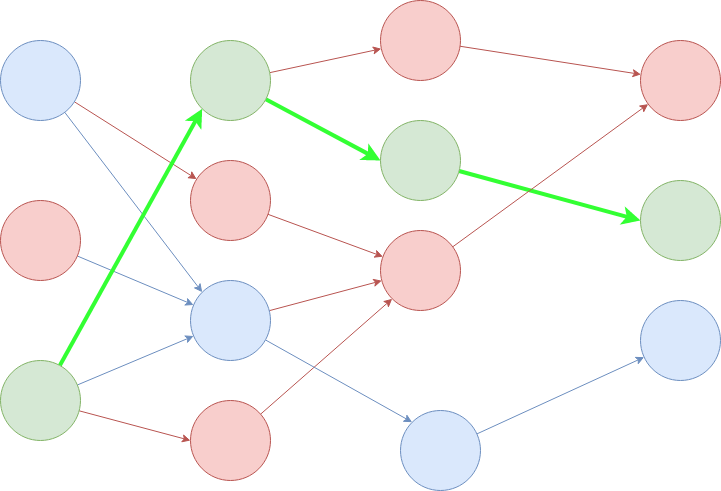
\includegraphics[scale=0.4]{deep_learning_schema}
	\captionof{figure}{Autoapprentissage Deep Learning}
	\label{fig1}
\end{center}

Les avantages de cette méthode sont qu'elle permet de sortir une bonne qualité sur les résultats obtenus. Elle permet aussi d'avoir une meilleure exécution sur des tâches de routine tout en gardant de très bon résultats ce qui est positif quand on sait que traiter des données non structurées n'est pas chose aisée. En effet, elle arrive à stocker des informations sous des formats désordonnés tels que documents, photos, mails. Cela montre bien la puissance du Deep Learning.\\

Bien entendu, il y a aussi des désavantages. On peut constater que ce type de modèle peut devenir très vite énergivore. De plus, le DL se focalise principalement sur une application. Or, il peut être intéressant d'étudier plusieurs applications similaires afin d'identifier des modèles plus poussés. C'est dans ce contexte que nous allons introduire le Federated Learning.
\pagebreak


\chapter{Federated Learning}

Avec la digitalisation des données et l'augmentation du nombre d'individus sur notre planète, on fait face à de nouveaux défis pour l'utilisation de toutes ces données présentes sur Internet. C'est la raison pour laquelle notre époque fait face à deux défis importants en termes d'avancées technologiques: \\
\begin{enumerate}
\item Le respect de la vie privée. L'un des plus importants est celui de la privatisation de ces données sur le web. Avec la protection des données (RGPD) promulguée en 2018, les données privées font entièrement partie de l'utilisateur, ces données ne peuvent pas être utilisées sans l'accord de leur propriétaire.
\item L'union fait la force, or, le traitement en silos des données de chaque entreprise freine énormément l'évolution des apprentissages de machine learning. En effet, en partageant les données entre différents secteurs, les algorithmes pourraient s'enrichir dans d'autres contextes afin de prendre de meilleures décisions en fonction du besoin de chaque application.
\end{enumerate}
Lors de mes recherches, j'ai lu la citation de Benjamin Merci, Responsable Digital Analytics : \\
\textit{«Sans connaissance de son audience, et sans hypothèses préalables solides, la Big data ne sert à rien».}\\
Benjamin Merci veut mettre en avant au travers de sa citation l'importance de la collecte des données. La masse d'information nécéssaire pour obtenir des apprentissages de qualité demande beaucoup de rigueur et d'expérience dans le domaine ciblé.\\
\pagebreak

Le Federated Learning peut est composé de deux familles bien distinctes :
\begin{enumerate}
\item La première est celle qui partage ses données sur un serveur centralisé.
\item La seconde est celle qui partage son modèle avec d'autres participants.
\end{enumerate}

\section{Apprentissage centralisé}

Pour commencer, la première méthode se base sur des modèles précédents comme le ML et le DL. Cette approche a besoin d'un large éventail de données pour pouvoir améliorer son échantillonnage et ressortir des données suivant un besoin spécifique au niveau du modèle.\\

Son fonctionnement consiste dans notre cas en la mise à disposition de plusieurs appareils (des robots présents dans l'article : "Data-Driven Federated Learning for Spatio-Temporal Predictions in Multi-Robot Systems") connectés sur un réseau à un serveur central.\\

Dans cet exemple, les robots doivent partager leurs données collectées afin de les fusionner. Cette fusion des données permet d’apprendre avec une meilleure perception de leur environnement global. Ce type d’approche ne fonctionne que si les données ne sont pas sensibles. Dans le cas contraire, il est important de trouver une solution pour anonymiser ou pseudonomyser les données afin de les protéger.\\

De nos jours, il existe des approches de pseudonomysation très abouties comme les méthodes de chiffrement. Au travers de l’article : "Extractop et gestion des connaissances", il est possible de constater l'utilité de la pseudonymisation en montrant la conservation d'informations sensibles à des fins scientifiques ou pour affiner des statistiques suivant un besoin. De plus, l’article reconnaît l'utilisation d'un chiffrement comme la méthode la plus courante pour la pseudonymisation. Cette méthode utilise un identifiant et un quasi-identifiant et les remplace par d'autres chiffres, ce qui rend l'identité cachée tout en permettant la ré-identification des informations aux détenteurs de la clé de déchiffrement. Le schéma 4.1 montre le fonctionnement du chiffrement d'une pseudonymisation.\\

\begin{center}
    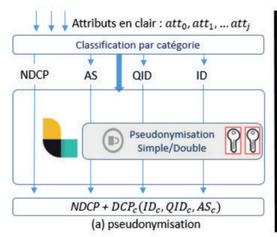
\includegraphics[scale=0.7]{pseudo}
    \captionof{figure}{Pseudonymisation}
    \label{fig1}
\end{center} 

Ainsi, la solution de l’apprentissage centralisé permet d’utiliser les technologies de plus en plus matures que sont le ML et le DL. Cependant, il faut être extrêmement vigilant à la protection des données d'apprentissage. Pour pallier ce problème de fuite des données sources, nous allons présenter le concept de partage des modèles d’apprentissages.
\pagebreak
\section{Modèle centralisé}

Dans cette section, nous allons détailler comment le FL peut améliorer la convergence des apprentissages sans forcément avoir besoin d'accéder aux données sources.

Dans ce contexte, le modèle centralisé permet de  partager ces modèles tout en faisant attention de ne pas divulguer des informations sensibles soumises à la protection des données. Cette approche de partage de modèle de prise de décision, comme nous le montre l'article "Federated Learning, Synthesis Lectures on Artificial Intelligence and Machine Learning", des entreprises ont décidé de la mettre en oeuvre à des fins de détection d'objets. Ils forment ainsi un ensemble de modèles puissants dans le but de répondre rapidement aux demandes des clients. Le travail des modèles est illustré à la fig 4.2.

\begin{enumerate}
\item Chaque participant va rechercher sur le serveur le modèle de détection d'objets.
\item Chaque participant utilise le modèle sur ses données en interne.
\item Chaque participant envoie ses paramètres sur le serveur via un protocole sécurisé.
\item Le serveur utilise les paramètres du modèle de chaque participant et met à jour son propre modèle de détection d'objets.
\end{enumerate}

\begin{center}
    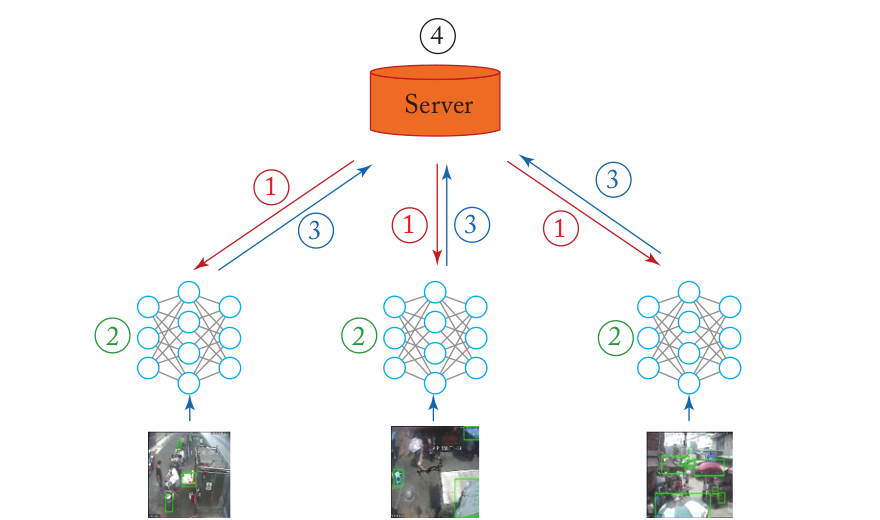
\includegraphics[scale=0.4]{fl_model_partage}
    \captionof{figure}{Modele partager}
    \label{fig1}
\end{center}

\pagebreak

Une autre approche peut être nécessaire pour mieux comprendre son fonctionnement. Le FL se déroule en plusieurs étapes, la formation fédérée est celle qui est la plus courante comme nous le montre la fig 4.3. Pour commencer, un appareil mobile se procure un modèle afin d'acquérir les données et les traiter en local. En second lieu, le modèle est soumis à de multiples mises à jour régulières en local afin d'être amélioré, celles-ci contiennent des données locales qui appartiennent à différents appareils séparés. Ensuite, les appareils mobiles téléchargent des informations d'un champ de vecteurs présent dans un cloud. En quatrième lieu, les modèles locaux effectuent une mise à jour moyenne au sein du cloud à modifier en fonction de ce qui est envoyé. Pour finir, ces étapes précédentes se répètent jusqu'à l'obtention d'un modèle avec une certaine performance ou qu'une date limite soit atteinte.

\begin{center}
	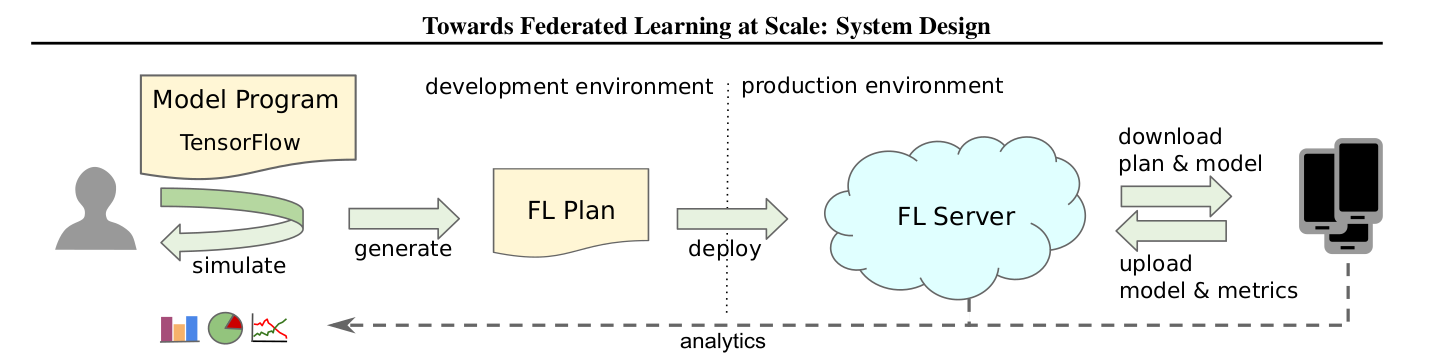
\includegraphics[scale=0.3]{mobile_schema_fl}
	\captionof{figure}{Schema FL}
	\label{fig1}
\end{center}

\section{Exploration des modèles}

Le FL est caractérisé par trois grands groupes qui surviennet régulièrement : le FL Horizontal, le FL Vertical et le Federated Transfer Learning. Les données stockées sont placées dans différents noeuds, celles ci ressemblent à une forme de matrice de caractéristiques. Les données sont composées de multiples instances, la partie horizontale est représentée comme un client, la partie verticale se distinque par les caractéristiques du client. Pour finir, on peut séparer le FL suivant le mode de partition des données.\\

\subsection{Horizontal FL}

Le FL Horizontal présente des chevauchement qui apparaissent entre les caractéristiques des données, réparties sur différents noeuds, malgré le fait que les données ne sont pas semblables sur l'espace d'échantillonnage. Les données du point de vue de l'échantillonage sont différentes dans les scénarios des appareils connectés à Internet et les appareils intelligents. Mais ils sont particulièrment similaire dans un espace de fonctionnalité. Les mises à jour, comme nous l'avons vu précédement dans le point du FL, faite de façon horizontal. En effet, la dimension d'entité est la même pour chaque donnée. Dans les applications médicales, une forte hausse de travail est nécessaire pour collecter un grand nombre de données. Car il est difficile voire inconcevable pour chaque hôpital de créer une banque de données à partager. Un réseau fédéral pour les hôpitaux construit par le FL permet d'améliorer le modèle(voir Fig 4.4).

\begin{center}
	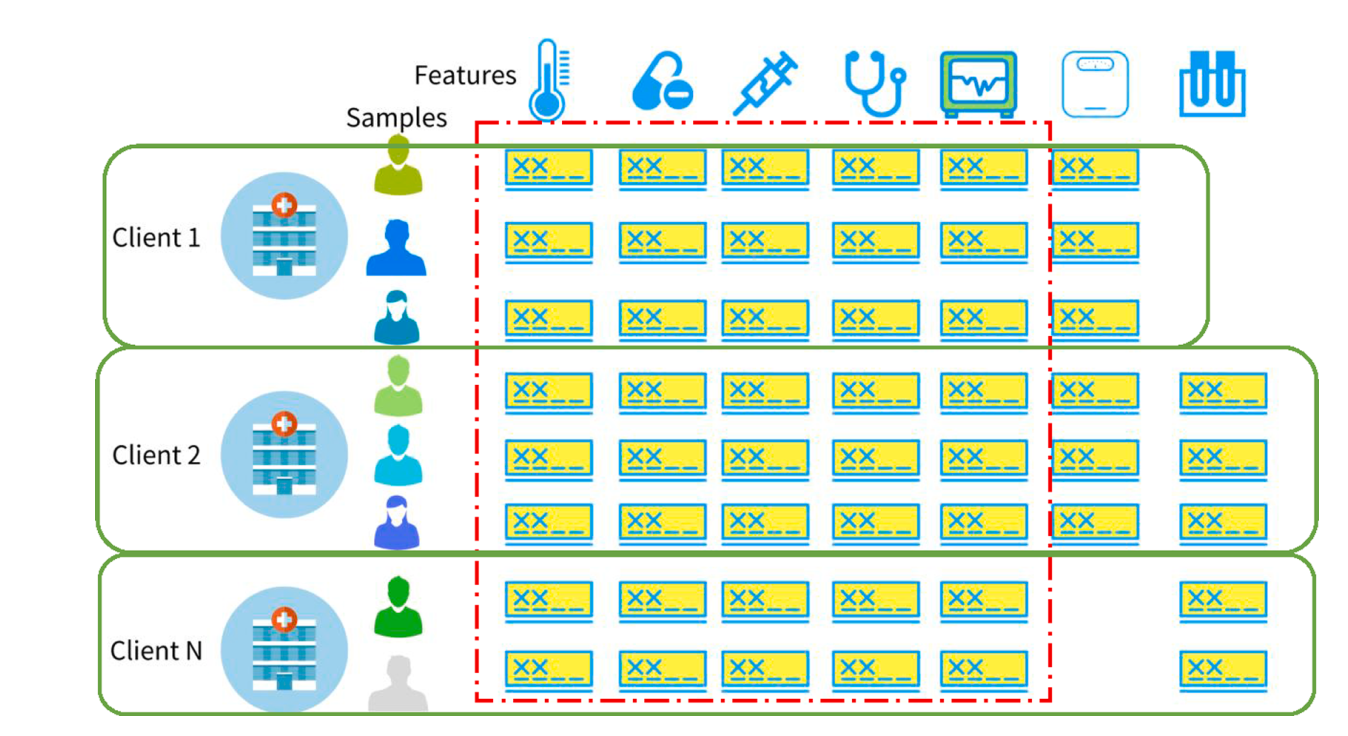
\includegraphics[scale=0.2]{fl_horizontal}
	\captionof{figure}{Horizontal FL}
	\label{fig1}
\end{center}


\subsection{Vertical FL}

Lorsque les données sont partitionnées, le FL vertical est plus approprié, chaque parties contient des données homogènes. Ce qui implique que les chevauchements se font en partie sur l'ID de l'échantillon alors qu'elle est différente dans l'espace fonctionnel. Prenons le cas d'un établissement médical qui souhaitent identifier des maladies, par exemple le diabète. Il peut être analysé selon certains critères tels que l'âge, le poids et les antécédants médicaux le type de diabète dont souffre un patient. De plus, les données de certaines applications qui comptent le nombre de pas effectués ou analysent la composition des plats ingérés peuvent être utilisées pour faciliter la reconnaissance. La figure 4.5 illustre très bien le FL vertical.

\begin{center}
	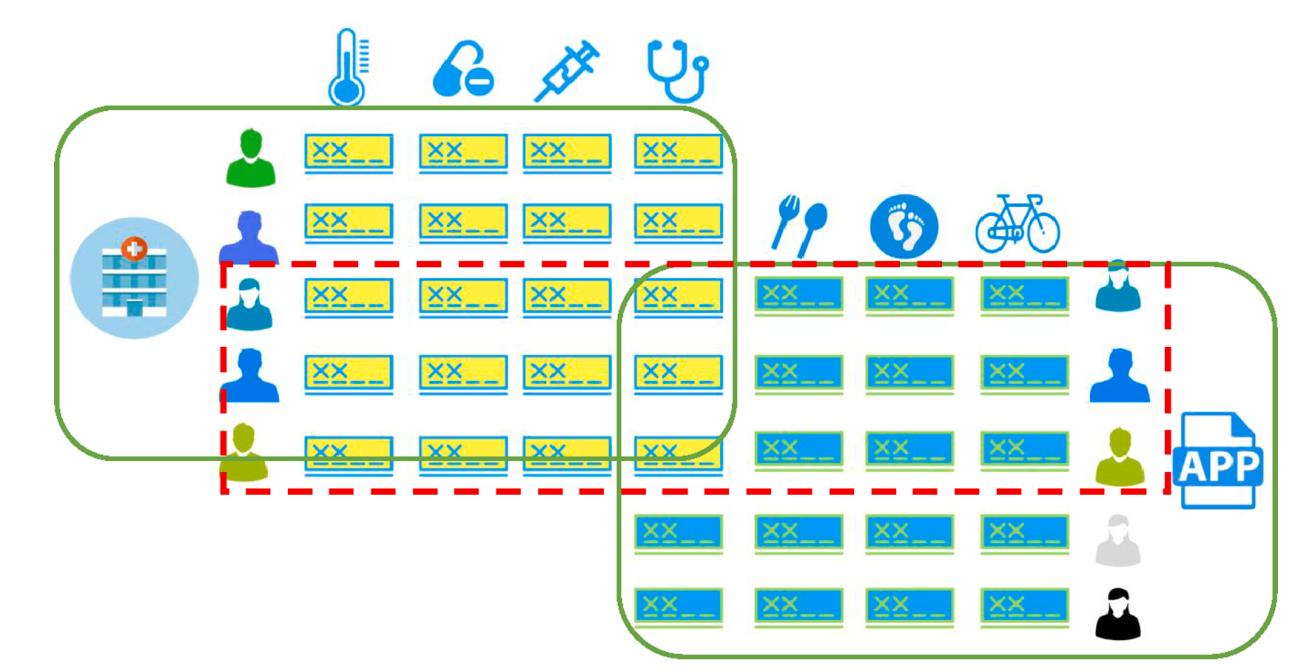
\includegraphics[scale=0.2]{fl_vertical}
	\captionof{figure}{Vertical FL}
	\label{fig1}
\end{center}


\subsection{Federated Transfer Learning (FTL)}

En comparaison des deux scénarios vus précédemment, dans la plupart des situations, sur les espaces d'échantillonnages ou d'entités, les données n'y sont pas partagées. Ce qui implique un manque d'étiquette et une mauvaise qualité des données. Le principe du FTL est de transféré les données d'un domaine vers un autre afin de réaliser de meilleurs résultats d'apprentissage. Ainsi, le FTL permet d'avoir une application étendue pour ce qui est des parties communes avec des intersections étroites. Pour un système de réseaux de neurones qui possèdent une technologie de cryptage homomorphique cela permet d'empêcher des fuites de confidentialités mais aussi de garder une très bonne précision. 

Dans le cadre d'une application avec le modèle FedHealth on a rassemblé un packet de données qui appartiennent à des organisations différentes via FL, le but étant d'avoir un service personnalisé pour des soins de santé. Sur la Fig 3.6, des informations sur le diagnostic et le traitement de certaines maladies peuvent être partagées avec un autre hôpital dans le but de faciliter des diagnostics. Les problèmes qui surviennent à l'heure actuelle dans le milieu de l'industrialisation sont les îlots de données et la protection de la vie privée. Le FTL offre la possibilité d'avoir un service de sécurité fiable pour la protection des données et la confidentialité des utilisateurs tout en cassant les barreaux des îlots de données.

\begin{center}
	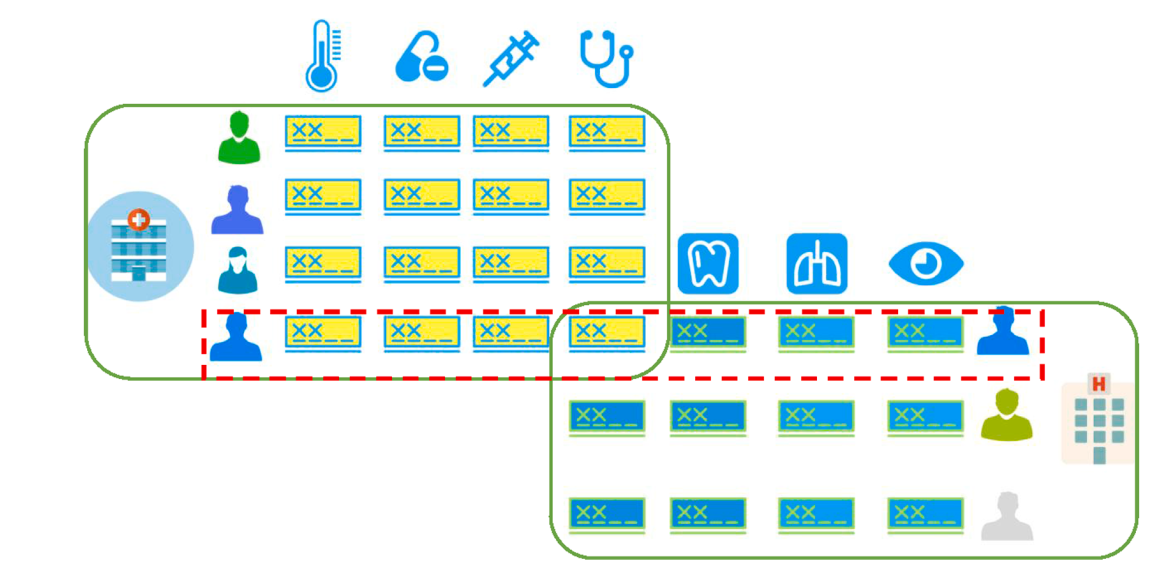
\includegraphics[scale=0.2]{fl_distribute}
	\captionof{figure}{FTL}
	\label{fig1}
\end{center}

En quelques mots, c'est un apprentissage automatique distribué qui permet d'entraîner un modèle mathématique avec un large groupe de données décentralisées qui se trouvent sur des appareils distants.\\

\section{Agrégation des modèles}

L'agrégation des modèles a pour but de fusionner des modèles similaires entre eux pour amplifier les pourcentages de succès des données en sorties.\\ 



\section{Conclusion FL}

L'esssor de l'industrie vient de l'utilisation du Federated Learning(FL) et c'est ainsi qu'elle a reussis à relever ses défis. L'utilisation d'îlots de données est la clé pour ces industries car le FL utilise un processus d'apprentissage automatique qui recourt à ces gros îlots. Cellui-ci utilise les concepts du ML et du DL pour pouvoir travailler avec ces grands échantillonnages de données. Des algorithmes de ML et de DL effectuent des calculs basés sur les données de leur application. L'objectif du FL est de pouvoir agréger des informations de diversses applications, ou de différents acteurs afin de générer un modèle plus abouti. Cette centralisation des données se fait généralement à l'aide d'un serveur centralisé comme le présente le schéma 4.7. Les données sont ainsi distribuées.
 
\begin{center}
	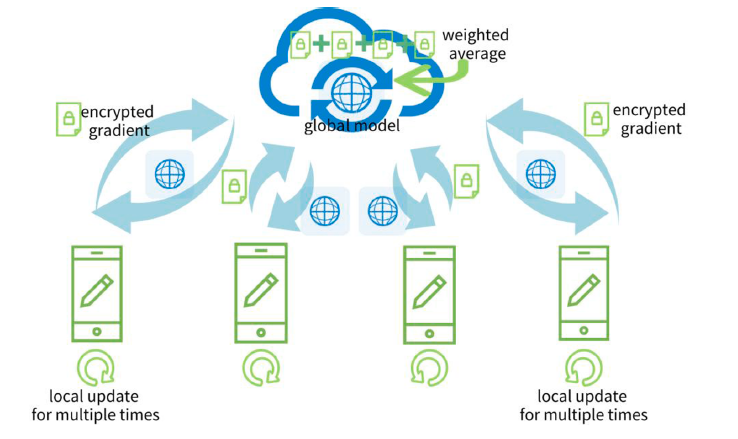
\includegraphics[scale=0.8]{fl}
	\captionof{figure}{Serveur centralisé}
	\label{fig1}
\end{center}






\chapter{Exemples d'utilisations}

Dans notre société, le FL peut être un atout majeur pour plusieurs secteurs comme le multimédia, la finance et les soins de santé. Plusieurs applications qui peuvent faciliter les employés dans leur travail de tous les jours ou encore aider à la reconnaissance de certaines maladies et bien entendu aider nos têtes blondes à améliorer et faciliter leur apprentissage afin qu'ils deviennent les hommes et les femmes de demain. Beaucoup de possibilités donc, et pour se faire une idée des domaines dnas lesquels il est possible d'utiliser le FL, voici quelques exemples. 


\section{Le Multimédia}

Le secteur du multimédia fait partie intégrante de notre quotidien et nous ne prêtons plus attention à toutes ces données misent sur le Web. L'article "Big and Personal: data and models behind Netflix recommendations" montre que le secteur du multimédia dispose de plusieurs données sur nos habitudes et nos préférences en termes de choix de visionnage. L'un des plus connus est Netflix. En effet cette société utilise nos données pour nous suggérer des choix parmi un large éventail de séries et de films. Ceux-ci se basent sur nos historiques, nos choix du moment. Une autre de leur fonctionnalité est de partager les séries/films que nos amis aiment. Ainsi l'utilisateur pourra être dirigé vers un visionnage susceptible de lui plaire. Ceci ne constitue qu'un exemple mais on peut imaginer plus loin cette utilisation. Pour cette raison, l'industrie a un enjeux capital dans tous ces îlots de données.\\

\section{La Finance}

Le secteur de la finance est très important et est soumis à des réglementations gouvernementales pour la protection des investisseurs contre la fraude et la mauvaise gestion, ainsi que pour la conservation de la confidentialité et la sécurités des données des utilisateurs. Dans le but de réduire les coûts et la charge de travail, des sociétés bancaires et financières exploitent les technologies modernes comme l'IA, les services de cloud et la technologie sur les téléphones mobiles pour assurer un service financier de qualité tout en respectant les réglementations gouvernemantales. Un cas bien particulier est le financement intelligent à la consomation, dont l'objectif vise à tirer parti des techniques de ML afin de proposer à chacun des services financiers sur mesure. Les données utilisées dans un crédit à la consommation regorgent d'informations sur les consommateurs comme le pouvoir d'achat, les préférences d'achats et aussi les caractéristiques du produit. Ces données peuvent être utilisée par diverses entreprises ou sociétés. Ainsi dans la figure 4.1, les informations de qualifications et le pouvoir d'achat d'un client peuvent être déduits de son épargne bancaire et de sa préférence d'achat sur des produits ou services. On fait face dans notre exemple à deux problèmes. Le premier est la protection de la vie privée des consommateurs et la sécurité des données barrière entre les banques, les réseaux sociaux, les sites d'e-commerce. Le deuxième est le stockage des données par trois sections hétérogènes, ce qui empêche le ML classique de fonctionner sur ces données hétérogènes. Le FL résout ces problèmes en scindant les données en 3 parties, sans les exposer. On peut aussi utiliser l'apprentissage par transfert pour examiner les données hétérogènes.

\begin{center}
	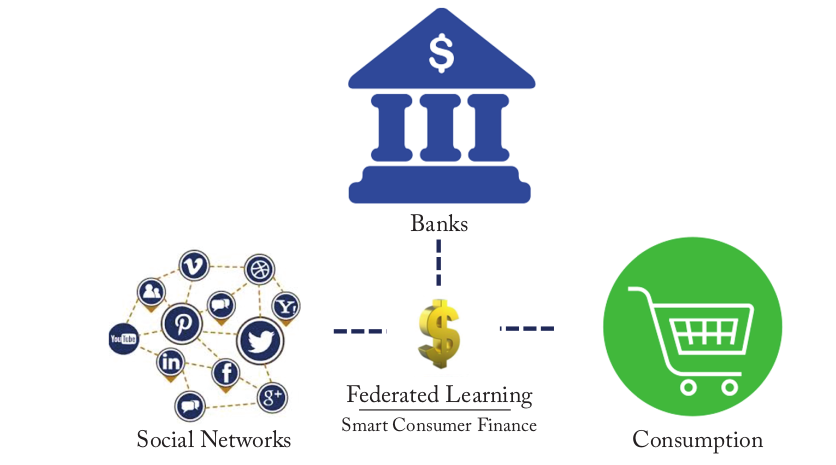
\includegraphics[scale=0.3]{finances}
	\captionof{figure}{FL dans une petite entreprise financière}
	\label{fig1}
\end{center}

\section{La santé}

Dans le domaine médical l'intervention de l'IA peut aider à réduire les coûts et les erreurs humaines dans les hôpitaux. En effet, un programme développé pour la biologie et la radiologie permet d'aider à poser un diagnostic sur des maladies cardiaques et identifier des cellules du cancer dans les premiers stades. Avec ces applications encourageantes de l'IA, beaucoup de fournisseurs de soins de santé tirent parti de l'IA pour améliorer et augmenter l'efficacité des soins pour les patients. Cependant, l'utilisation de cette technologie n'en est qu'à ses débuts car des erreurs sont déjà survenues à la suite d'un mauvais diagnostic. Le plus gros problème dans ce domaine est la quantité d'informations nécessaires pour diagnostiquer précisément des symptômes sur un patient. Par exemple pour diagnostiquer un rhume, il faut plusieurs caractéristiques provenant de différentes sources, ainsi que les symptômes de la maladie.

Pour cette raison, les institutions médicales doivent partager leur données en respectant les règles de la protection de la vie privée. Par après, on peut former un grand ensemble de données qui fonctionne bien mieux que des données provenant d'un seul établissement. Si on fusionne le FL et l'apprentissage par transfert, cela promet une bonne solution pour réaliser cet objectif. L'apprentissage fédéré permet de former un modèle partagé sans exposition et échange de données propres à un patient. Ensuite, les techniques d'apprentissage par transfert aident à élargir l'échantillonnage et améliorent les performances de partages des données. Pour terminer, l'apprentissage par transfert joue un rôle considérable dnas le développement des systèmes médicaux. Si plusieurs institutions médicales établissent une bonne base de données grâce à l'apprentissage fédéré, l'avenir de l'IA dans le domaine de la santé peut avoir un net avantage sur les maladies. 

\begin{center}
	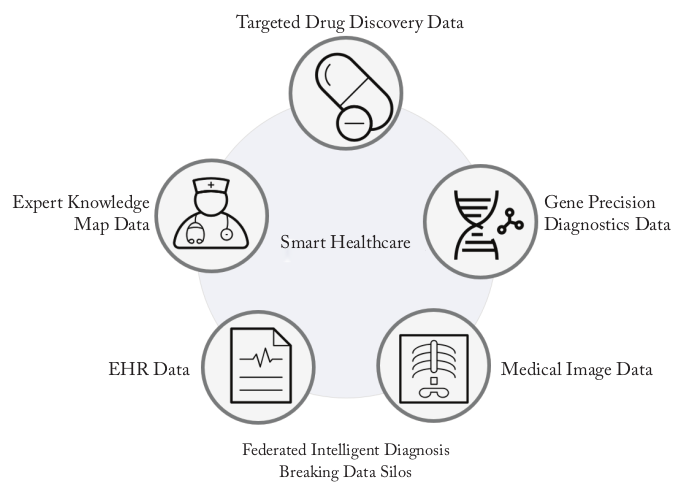
\includegraphics[scale=0.5]{medic}
	\captionof{figure}{FL Diagnostique }
	\label{fig1}
\end{center}

\chapter{Conclusion}

Après ces recherches, le Machine Learning manipule ainsi les gros volumes de données présents sur la toile. Il traite ce volume grâce à une modèle programmé et soumis à plusieurs tests. Le Deep Learning quant à lui, va plus en profondeur avec son système de neurone qui grâce à une image peut en ressortir des informations comme la présence d'un animal sur une photo. Le Federated Learning exploite les données via des serveurs sécurisés et dont les données sont décentralisées. Il gagne en performance et en vitesse de calcul. On peut imaginer un monde futuriste dans lequel la détection de symptômes pourra être détectée par un simple scan du corps. Détecter des infractions par l'intermédiaire de plusieurs caméras déjà présentes dans les commerces et les rues.  



\begin{thebibliography}{9}

	\bibitem{lamport94}
	  Leslie Lamport,
	  \emph{A Document Preparation System}.
	  Addison Wesley, Massachusetts,
	  2nd Edition,
	  1994.
	  
	\bibitem{LiliYuxiTseLin}
	  Li Li, Fan de Yuxi, Mike Tse, Kuo-Yi Lin,
	  \emph{A review of applications in federated leaning}.
	  Comuters and Industrial Engineering,
	  Volume 149,
	  November 2020,
	  106854
	  
	  \bibitem{FL_synthesis}
	  Qiang Yang, Yang Liu, Yong Cheng, Yan Kang, Tianjian Chen, Han Yu
	  \emph{Federated Learning, Synthesis Lectures on Artificial Intelligence and Machine Learning}.
	  Ronald J. Brachlan, Francesca Rossi and Peter Stone,
	  Morgan and Claypool publishers,
	  Series Editors
	  December 2019
	  
	  \bibitem{FL doc prof}
	  Keith Bonawitz, Hubert Eichner, Wolfgang Grieskamp, Dzmitry Huba, Alex Ingerman, Vladimir Ivanov, Chloé Kiddon , Jakub Konecny,  Stefano Mazzocchi, H. Brendan McMahan, Timon Van Overveldt, David Petrou, Daniel Ramage, Jason Roselander
       \emph{TOWARDS FEDERATED LEARNING AT SCALE: SYSTEM DESIGN} 22 Mars 2019  
	  	  
	  \bibitem{Netflix}
	  Xavier Amatriain
	  \emph{Big and Personal: data and models behind Netflix recommendations}.
	  Augustus 2013
	  
	  \bibitem{pseudonomysation}
	  Jérôme Azé.
	  \emph{Extractop, et gestion des connaissances}
	  \url{https://books.google.fr/books?hl=fr&lr=&id=dOEaEAAAQBAJ&oi=fnd&pg=PA419&dq=pseudonymisation+des+donn%C3%A9es&ots=EBRSMlwkfU&sig=Ss5Ik0PWRg_lR8K7-MVDwXPf2jA&redir_esc=y#v=onepage&q=pseudonymisation%20des%20donn%C3%A9es&f=false}
	  
	  \bibitem{Machine Learning supervised}
	  Hausmane Issarane.
	  \emph{Apprentisage Supervise}
	  \url{URL : https://analyticsinsights.io/5-apprentissage-supervise/} Consulté le 12/08/2021
		  
	  \bibitem{Deep Learning}
	  Retengr.
	  \emph{Deep Learning : définition, applications, avantages et inconvénients.}
	  \url {https://www.retengr.com/2021/01/22/deep-learning-definitions-applications-avantages-inconvenients/}
	  Consulté le 10/08/2021
	  
	\bibitem{bigdata}
	Bastien L.
	\emph{Machine Learning et Big Data.}
	\url {https://www.lebigdata.fr/machine-learning-et-big-data} Consulté le 14/06/2021
	
	\bibitem{ML Non supervise}
	Afshine Amidi et Shervine Amidi.
	\emph{Pense-bête d'apprentissage non-supervise.}
	\url{https://stanford.edu/~shervine/l/fr/teaching/cs-229/pense-bete-apprentissage-non-supervise} Consulté le 14/08/2021

\end{thebibliography}


%\label{TensorFlow : https://www.lebigdata.fr/tensorflow-definition-tout-savoir}

%Citeseer citeseer.ist.psu.edu,Google Scholar scholar.google.com,ScienceDirect www.sciencedirect.com,ACM Digital Library portal.acm.org,IEEE Digital Library www.computer.org/portal/site/csdl/index.jsp
 


\begin{appendix}
\chapter{Annexe}
 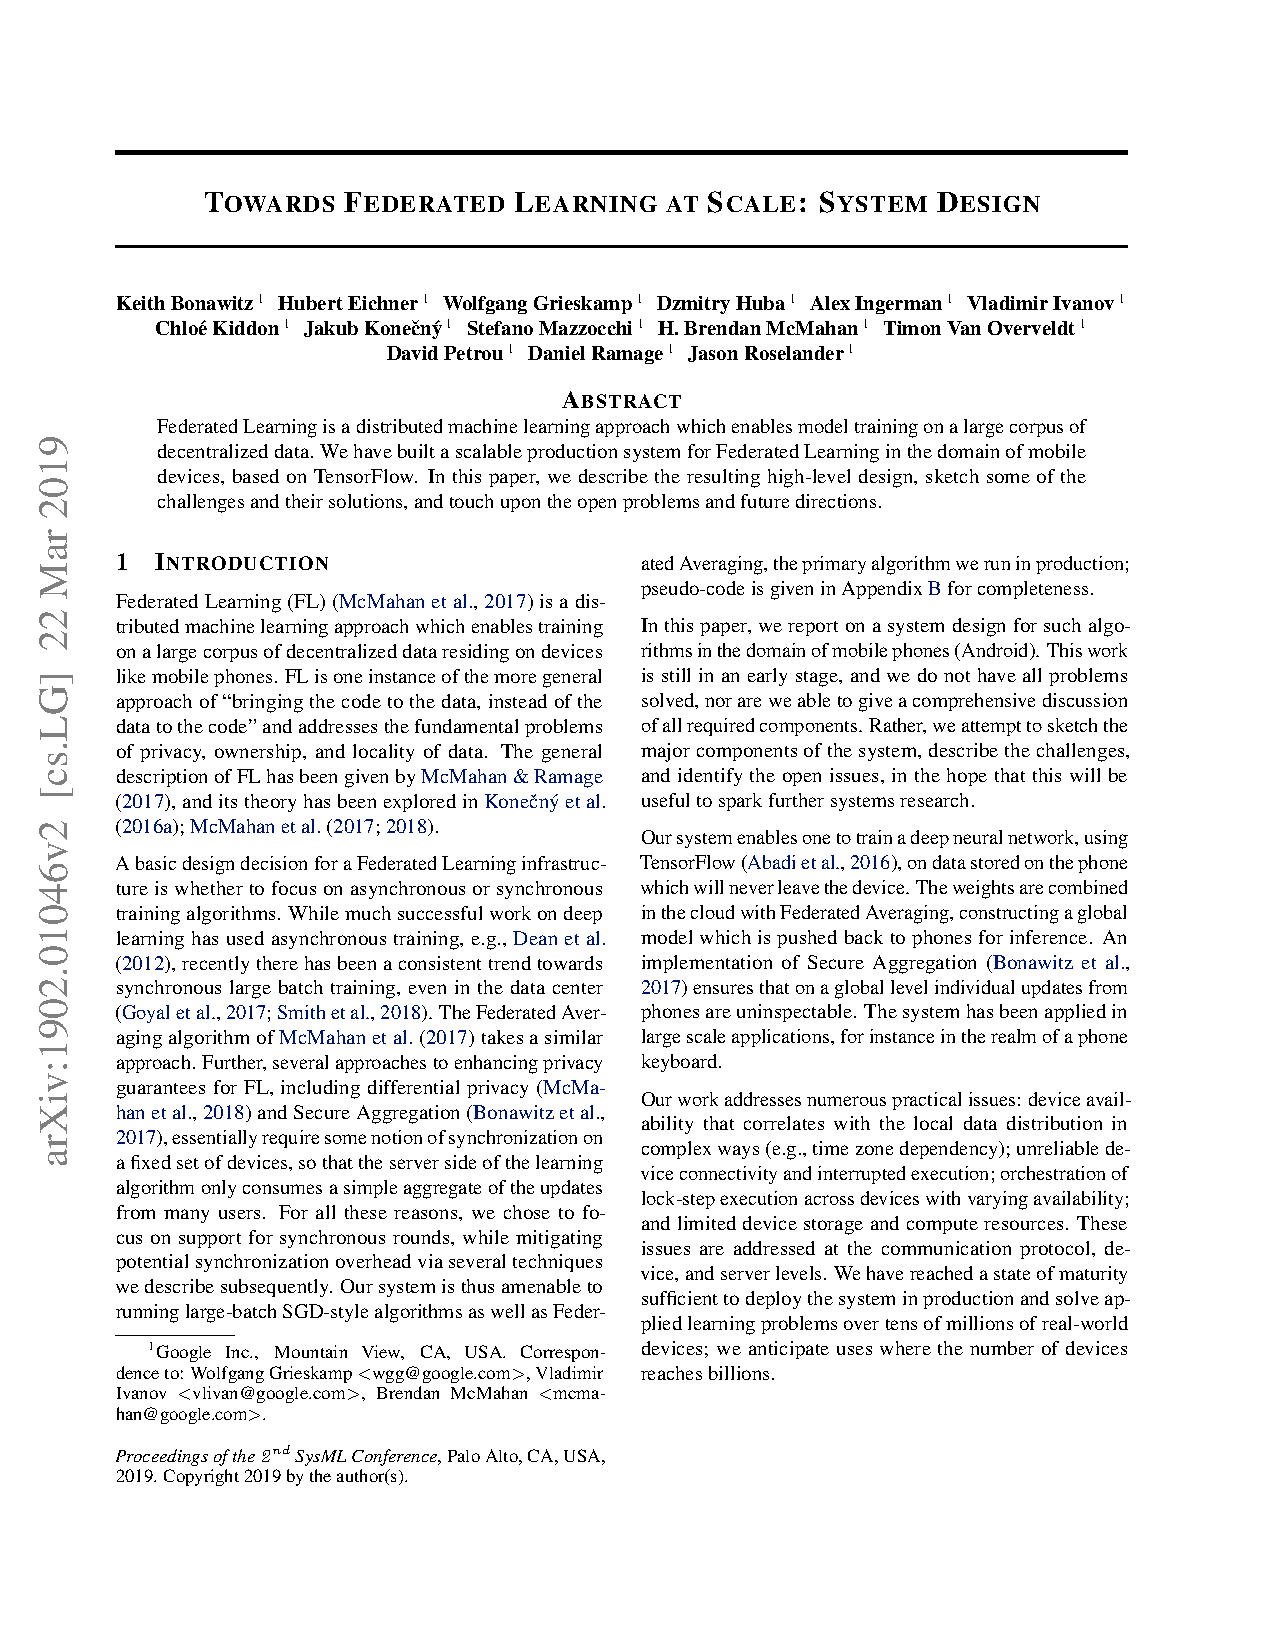
\includepdf{pdf/federate_learning_en.pdf}
\end{appendix}

\end{document}
